\documentclass{article}

\usepackage{graphicx}
\usepackage{tikz}
\usepackage{tikzsymbols}
\usetikzlibrary{calc,patterns,shapes.geometric}
\pagestyle{empty}
\usepackage[margin=0pt]{geometry}
\geometry{papersize={14in,12in}}

\def\centerarc[#1](#2)(#3:#4:#5){\draw[#1] ($(#2)+({#5*cos(#3)},{#5*sin(#3)})$) arc (#3:#4:#5);}

\begin{document}
	\begin{figure}
		\centering
		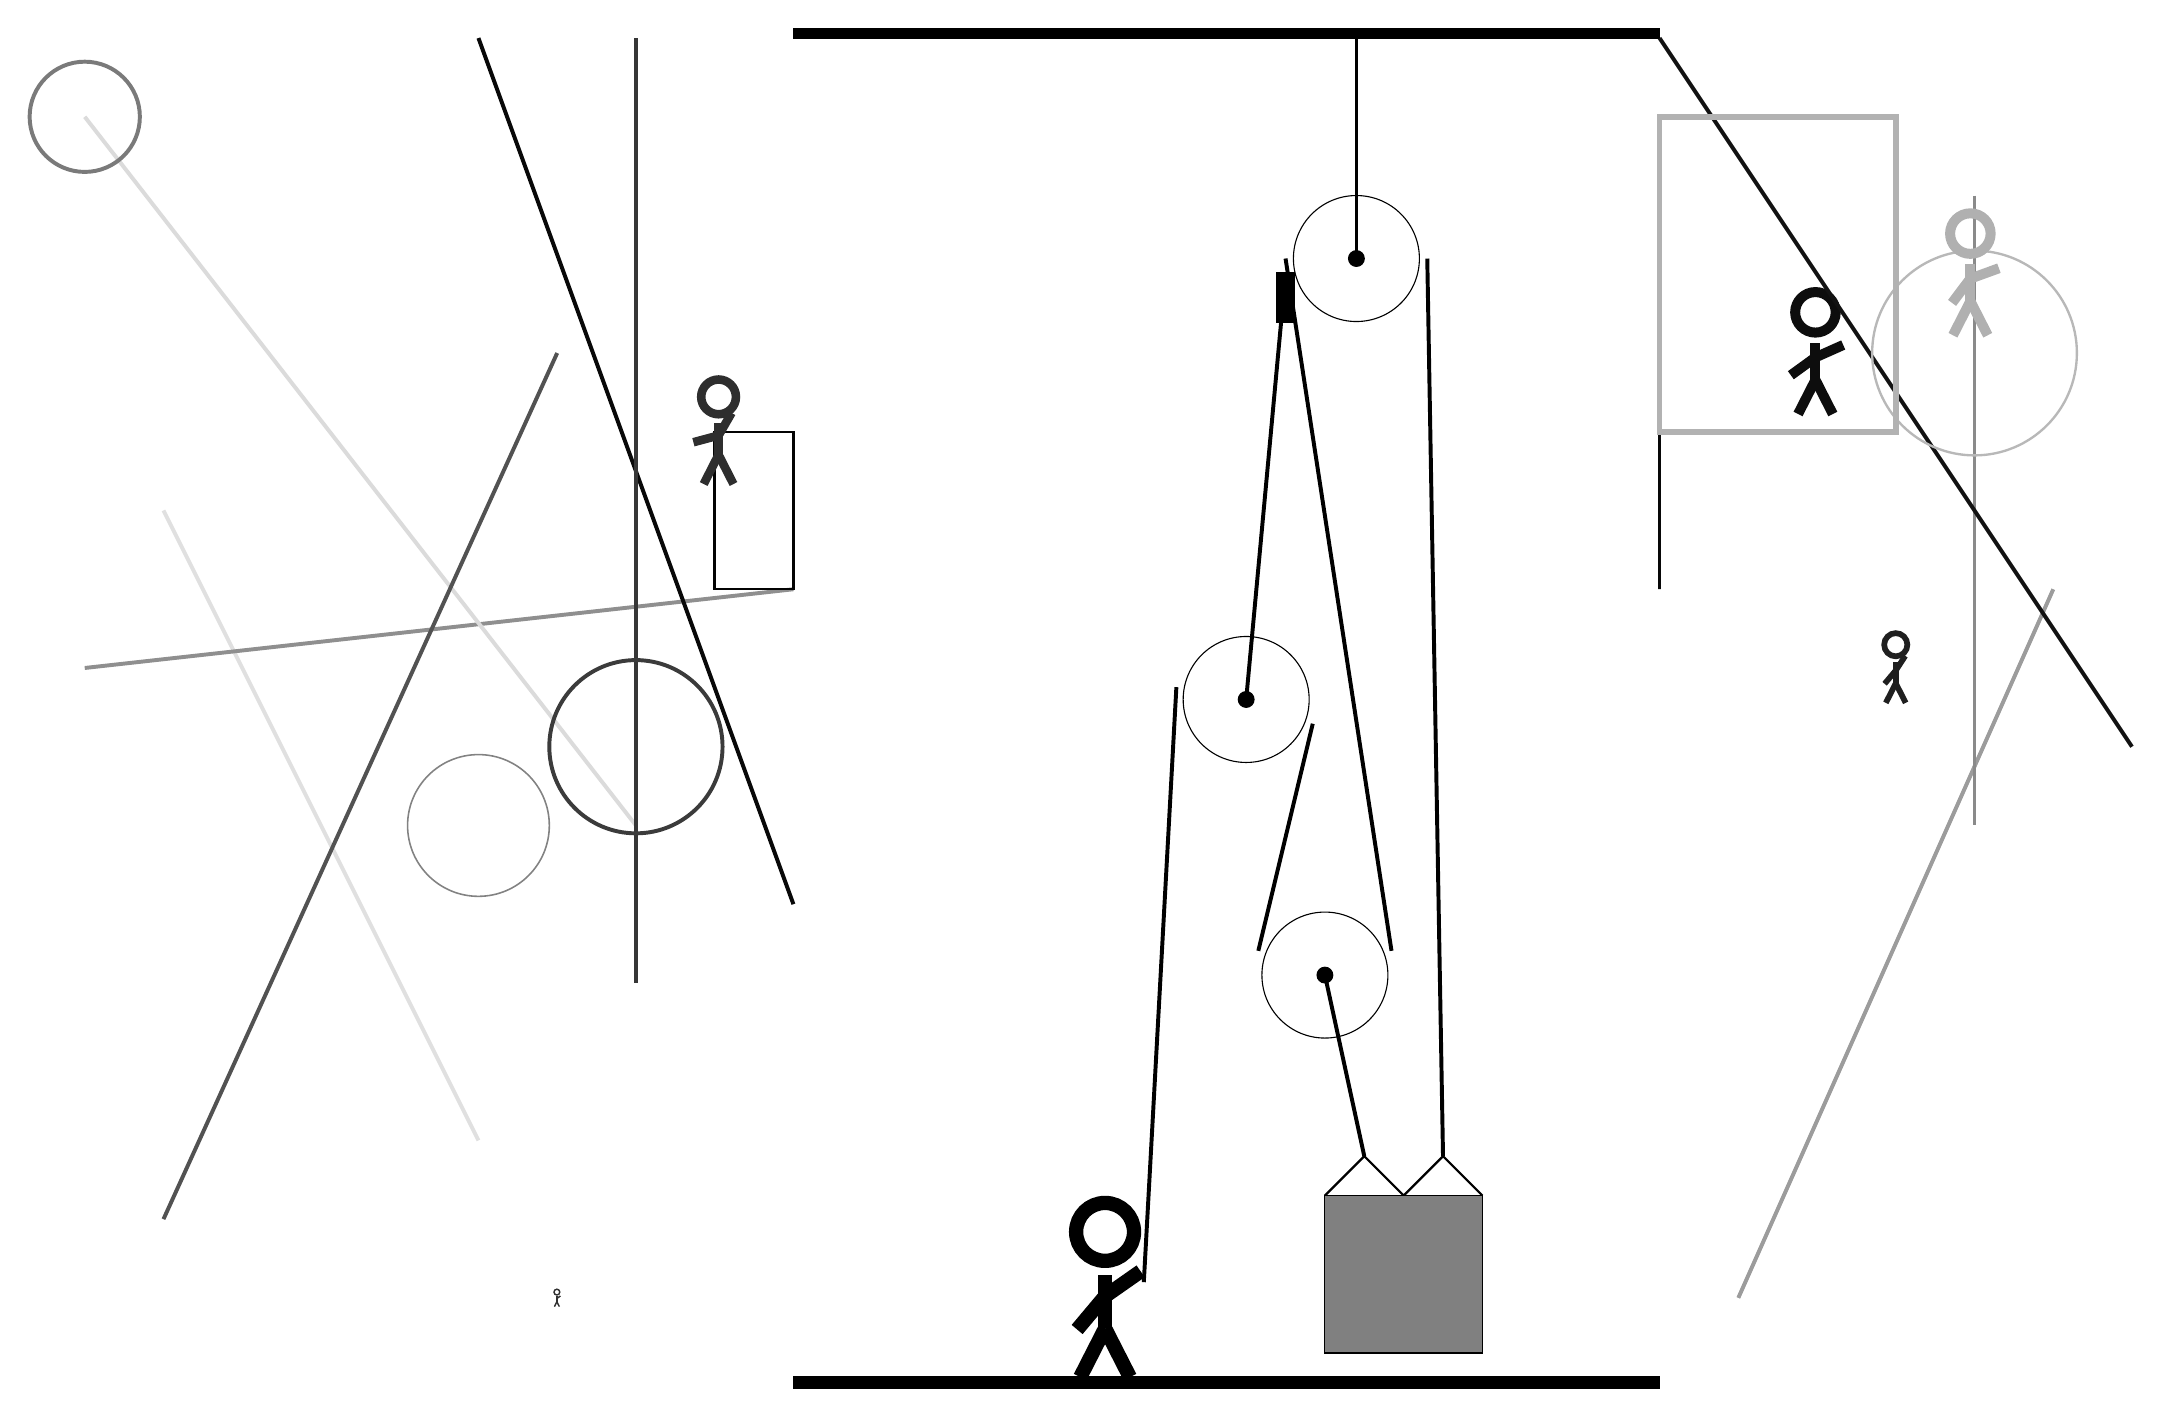
\begin{tikzpicture}
			%%%%% START %%%%%
			
			\draw[fill=black] (-6, 14) rectangle (5, 14.125);
			
			\draw (-0.25, 5.6) circle (0.8);
			\draw[fill=black] (-0.25, 5.6) circle (0.1);
			
			\draw[line width=0.5mm, color=black!39](6, -2) -- (10, 7);
			
			\node[line width=0.2mm, color=black!88] at (8, 6) {\Strichmaxerl[4][50][57]};
			\draw[line width=0.5mm, color=black!12](-10, 0) -- (-14, 8);
			\node[line width=0.7mm, color=black!95] at (7, 10) {\Strichmaxerl[7][36][24]};
			\draw[line width=0.5mm, color=black!44](-6, 7) -- (-15, 6);
			\draw[line width=0.5mm, color=black!14](-8, 4) -- (-15, 13);
			\draw[line width=0.5mm, color=black!46](9, 12) -- (9, 4);
			\draw[line width=0.5mm, color=black!97](-10, 14) -- (-6, 3);
			\draw [line width=0.6mm, color=black!43](-10, 4) circle (0.0);
			\draw[line width=0.5mm, color=black!68](-9, 10) -- (-14, -1);
			\draw[line width=0.3mm, color=black!99] (-6, 7) rectangle (-7, 9);
			
			\node[line width=0.4mm, color=black!82] at (-7, 9) {\Strichmaxerl[6][15][60]};
			\draw[line width=0.4mm, color=black!97] (5, 7) rectangle (5, 12);
			
			\draw[line width=0.6mm, color=black!79] (-8, 2) rectangle (-8, 14);
			\draw [line width=0.2mm, color=black!49](-10, 4) circle (0.9);
			\draw [line width=0.5mm, color=black!52](-15, 13) circle (0.7);
			\draw[line width=0.5mm, color=black!93](5, 14) -- (11, 5);
			
			\draw [line width=0.3mm, color=black!28](9, 10) circle (1.3);
			\draw[line width=0.7mm, color=black!30] (5, 9) rectangle (8, 13);
			
			\node[line width=0.3mm, color=black!31] at (9, 11) {\Strichmaxerl[7][53][20]};
			\draw [line width=0.5mm, color=black!77](-8, 5) circle (1.1);
			\node[line width=0.7mm, color=black!81] at (-9, -2) {\Strichmaxerl[1][90][36]};
			
			\draw (0.75, 2.1) circle (0.8);
			\draw[fill=black] (0.75, 2.1) circle (0.1);
			
			\draw (1.15, 11.2) circle (0.8);
			\draw[fill=black] (1.15, 11.2) circle (0.1);
			\draw[very thick] (1.15, 11.2) -- (1.15, 14);
			
			\draw[thick]  (0.75, -0.7) -- (1.25, -0.2) -- (1.75, -0.7) -- (2.25, -0.2) -- (2.75, -0.7);
			\draw[fill=black!50] (0.75, -0.7) rectangle (2.75, -2.7);
			
			\draw[line width=0.5mm] (-0.25, 5.6) -- (0.25, 11.0);
			\draw[line width=0.5mm, fill=black](0.15, 10.4) rectangle (0.35, 11.0);
			\draw[line width=0.5mm] (-1.55, -1.8) -- (-1.1363, 5.7562);
			\centerarc[line width=0.5mm](-0.25, 5.6)(-20:170:0.9);
			\draw[line width=0.5mm] (0.5957, 5.2922) -- (-0.0957, 2.4078);
			\centerarc[line width=0.5mm](0.75, 2.1)(160:380:0.9);
			\draw[line width=0.5mm] (1.5957, 2.4078) -- (0.25, 11.2);
			\draw[line width=0.5mm](0.75, 2.1) -- (1.25, -0.2);
			\centerarc[line width=0.5mm](1.15, 11.2)(0:180:0.9);
			\draw[line width=0.5mm] (2.05, 11.2) -- (2.25, -0.2);
			
			\node at (-2, -1.9) {\Strichmaxerl[10][50][35]};
			
			\draw[fill=black] (-6, -3) rectangle (5, -3.15);
			
			%%%%% END %%%%%
		\end{tikzpicture}
	\end{figure}	
\end{document}